% D04-010. PDR-05 §2, физический контракт.
\section{Направленность и применимость измерительного органа}
\label{sec:ch5_direction_validity}
\conceptsource{Статья 5 «Статистически обоснованная подготовка
данных и инженерная проверка органов направления мощности»,
раздел 2. Выход направления отделён от применимости;
показана связь с блокировкой БАВР и условность обозначения
обратного состояния для подпороговых токов.}

При снижении напряжения на секции шин существенно
не только наличие аварийного процесса, но и его
положение относительно рабочего ввода.
После потери внешнего питания двигательная нагрузка
может переходить в групповой выбег и кратковременно
отдавать энергию в питающую сеть.
При повреждении на стороне нагрузки направление
подпитки может оставаться прямым.
Эти режимы требуют разного поведения
блокирующих органов в логике БАВР.

Общие принципы измерения направления мощности
рассмотрены в главе~\ref{ch:bavr_modernization}.
Здесь фиксируется целевой ответ,
относительно которого далее сопоставляются
аналитические и нейросетевые органы.
Такое определение предшествует сравнению
их численных показателей.

\subsection{Выход направления в принятой логике БАВР}
\label{sec:ch5_direction_target}
\conceptsource{Статья 5, принятая полярность прямого/обратного
состояния и назначение блокирующего сигнала. Это конкретный
контракт исследования, не универсальная маркировка всех терминалов.}

\iffalse
(Примечание автора: Стоит писать не обратный поток, а «обратное направление», да и не прямой поток, а тоже направление, главное не писать постоянно направление, а всё же и синонимы каике-то, если потребуется.)
(Примечание автора: Ок, принято)
\fi
\authorreviewnote{AA141}

Прямое направление соответствует передаче активной мощности
от питающей сети к шинам нагрузки.
В принятой логике ему соответствует
положительный выход направления и формирование
блокирующего признака БАВР.
Обратное направление при выбеге относится
к отсутствию этого блокирующего признака.

При этом нулевой выход исследуемого органа
охватывает также подпороговый ток
при достаточном опорном напряжении.
Такой ответ означает несрабатывание блокирующего
органа, а не обязательно физически измеренный
обратную передачу энергии.
Это различие учитывается при подготовке меток
и рассмотрении границ чувствительности.

При нулевом признаке применимости передаётся сообщение,
что выходом направления пользоваться нельзя. По решению автора
этот признак предусматривается для обработки в общей блокирующей
логике БАВР. Выбор между блокировкой отдельной секции и общей
блокировкой относится к дальнейшему проектированию автоматики.
В настоящем исследовании проверяются выходы измерительного органа.

Ошибки соединения каналов при экспертном просмотре распознавались
по самим осциллограммам. Примером служит перестановка фаз B и C
только в одной группе измерений, нарушающая соответствие токов
и напряжений. Такие интервалы отмечал специалист. Это не означает,
что для каждого дефекта уже реализовано отдельное автоматическое правило.

Рабочий угол секторной характеристики
может смещать её границу относительно
линии нулевой активной мощности.
Поэтому положительный выход такой характеристики
и отдельно измеренный знак активной мощности
рассматриваются раздельно.

Отсутствие блокировки по данному выходу
является одним из условий работы БАВР.
Оно не заменяет проверки остальных условий
переключения и само по себе
не является командой выключателю.

% D06-005 R5-02 BEGIN
\ifdefined\AuthorReview
\par\smallskip\begingroup\small\raggedright\color{red!60!black}
\noindent\textbf{Примечание рецензента [R5-02], физическая постановка.} Нужно определить смысл выхода неприменимости для внешней логики БАВР: сохраняется блокировка, используется другой орган либо решение передаётся отдельной логике. Сейчас описаны прямое и нулевое состояния, но действие при VALID=0 остаётся открытым. Самостоятельно выбирать его нельзя. Достаточно согласованного автором объяснения или явной границы, что здесь проверяется измерительный орган, а правило обработки его отказа ещё не задано. Это влияет и на инженерную трактовку «лишнего отказа».\par\endgroup\smallskip
\fi
% D06-005 R5-02 END
\ifdefined\AuthorReview
\par\smallskip{\small\color{blue!60!black}\noindent\textbf{Ответ D06-006 на R5-02 (10.11.2026).} По уточнению автора сигнал непригодности передаётся внешней блокирующей логике. Выбор общей или посекционной блокировки оставлен проектированию БАВР; метки не менялись.\par}\smallskip
\fi
(Примечание автора: Ок, закрываем вопрос выше) 

\iffalse
(Примечание автора: При обнулении сигнала о валидности данных предлагается выдавать это во вне в качестве общей блокировки. Дальше БАВР своей внутренней логикой будет это конвертировать как требуется, либо ставить 1 по РНМ и не давать работать БАВР по этой секции, или вообще вызывать общую блокировку, по аналогии с неисправностями ТТ, но это под вопросом. В общем данный вопрос здесь глубоко не рассматривается, прост выдаётся сигнал о том, что в данном случае значения с органа нельзя считать за валидные, что-то аналогичное с метками в новых версиях МЭК 61850 о сомнительности / некорректности данных, они там как-то иначе называются, конечно. А уж как по ним будет работать логика выше – отдельный вопрос.)
(Примечание автора: Ок, закрываем вопрос)
\fi
\authorreviewnote{AA142}

\subsection{Достаточность измерительного контекста}
\label{sec:ch5_applicability_target}
\conceptsource{Статья 5. Неприменимость при недостаточной
опорного напряжения или дефектах измерений; отдельно исключение
файла без минимального состава и маскирование временного интервала.}

Направление может не определяться,
если имеющихся измерений недостаточно
для достоверного решения.
Характерный случай связан с глубокой потерей
опорного напряжения после исчерпания
используемой предыстории.
В рассматриваемой постановке принят порог
$0{,}05U_{\text{ном}}$.
Для органа с памятью учитывается
не только текущий сигнал,
но и сохранённая опорная величина.

Другую группу образуют дефекты измерительного
тракта. К ним относятся нарушение фазировки,
ошибочная полярность, использование неподходящих
цепей напряжения и записи отдельных
наладочных испытаний.
Согласованная циклическая перестановка
всех токов и напряжений сама по себе
не относится к таким дефектам.

\iffalse
(Примечание автора: Надо бы чуть лучше пояснить примеры. Ведь здесь речь о том, что фазы В и С перепутали местами например, и что-то подобное, но опять же, в жёсткой логике это не прописано, а лишь эксперт при разметке сам размечал, что он считает не валидным.)
(Примечание автора: Ок, закрываем вопрос)
\fi
\authorreviewnote{AA143}

Различаются отсутствие нужного состава
каналов во всём файле и временная
неприменимость при сохранённых измерениях.
В использованной подготовке файл исключается,
если нельзя сформировать минимальный
базис из двух токов и двух напряжений.
Его исключение не создаёт автоматически
обучающую цель неприменимости.

Если минимальный состав присутствует,
непригодное состояние может относиться
лишь к части записи.
Тогда отдельно задаётся признак применимости
для соответствующего временного интервала.
Направлению на нём не присваивается
искусственное прямое или обратное значение.
Порог малого тока при нормальном напряжении
не смешивается с этой ситуацией.

\subsection{Два выхода интеллектуального РНМ}
\label{sec:ch5_twohead_target}
\conceptsource{Статья 5, двухголовая постановка и рисунок 1.
Различаются расчёт двух оценок общей моделью и условное
использование направления при допустимом контексте.}

\iffalse
(Примечание автора: Хмм… Вот тут ты говоришь про два выхода, а идею неприменимости озвучиваешь выше. Как-то не бьётся и для читателя раньше не совсем понятна та концепция. Её надо раньше как-то лучше бы описать, про два выхода.)
(Примечание автора: Ок, закрываем вопрос)
\fi
\authorreviewnote{AA144}

Для нейросетевого органа вводятся две
целевые величины. Первая обозначает
применимость измерительного контекста,
вторая прямое направление при его применимости.
Обе оценки формируются общей моделью
с отдельными выходными частями.
Смысл их совместного использования
показан на рисунке~\ref{fig:ch5_twohead_logic}.

\begin{figure}[htbp]
 \centering
 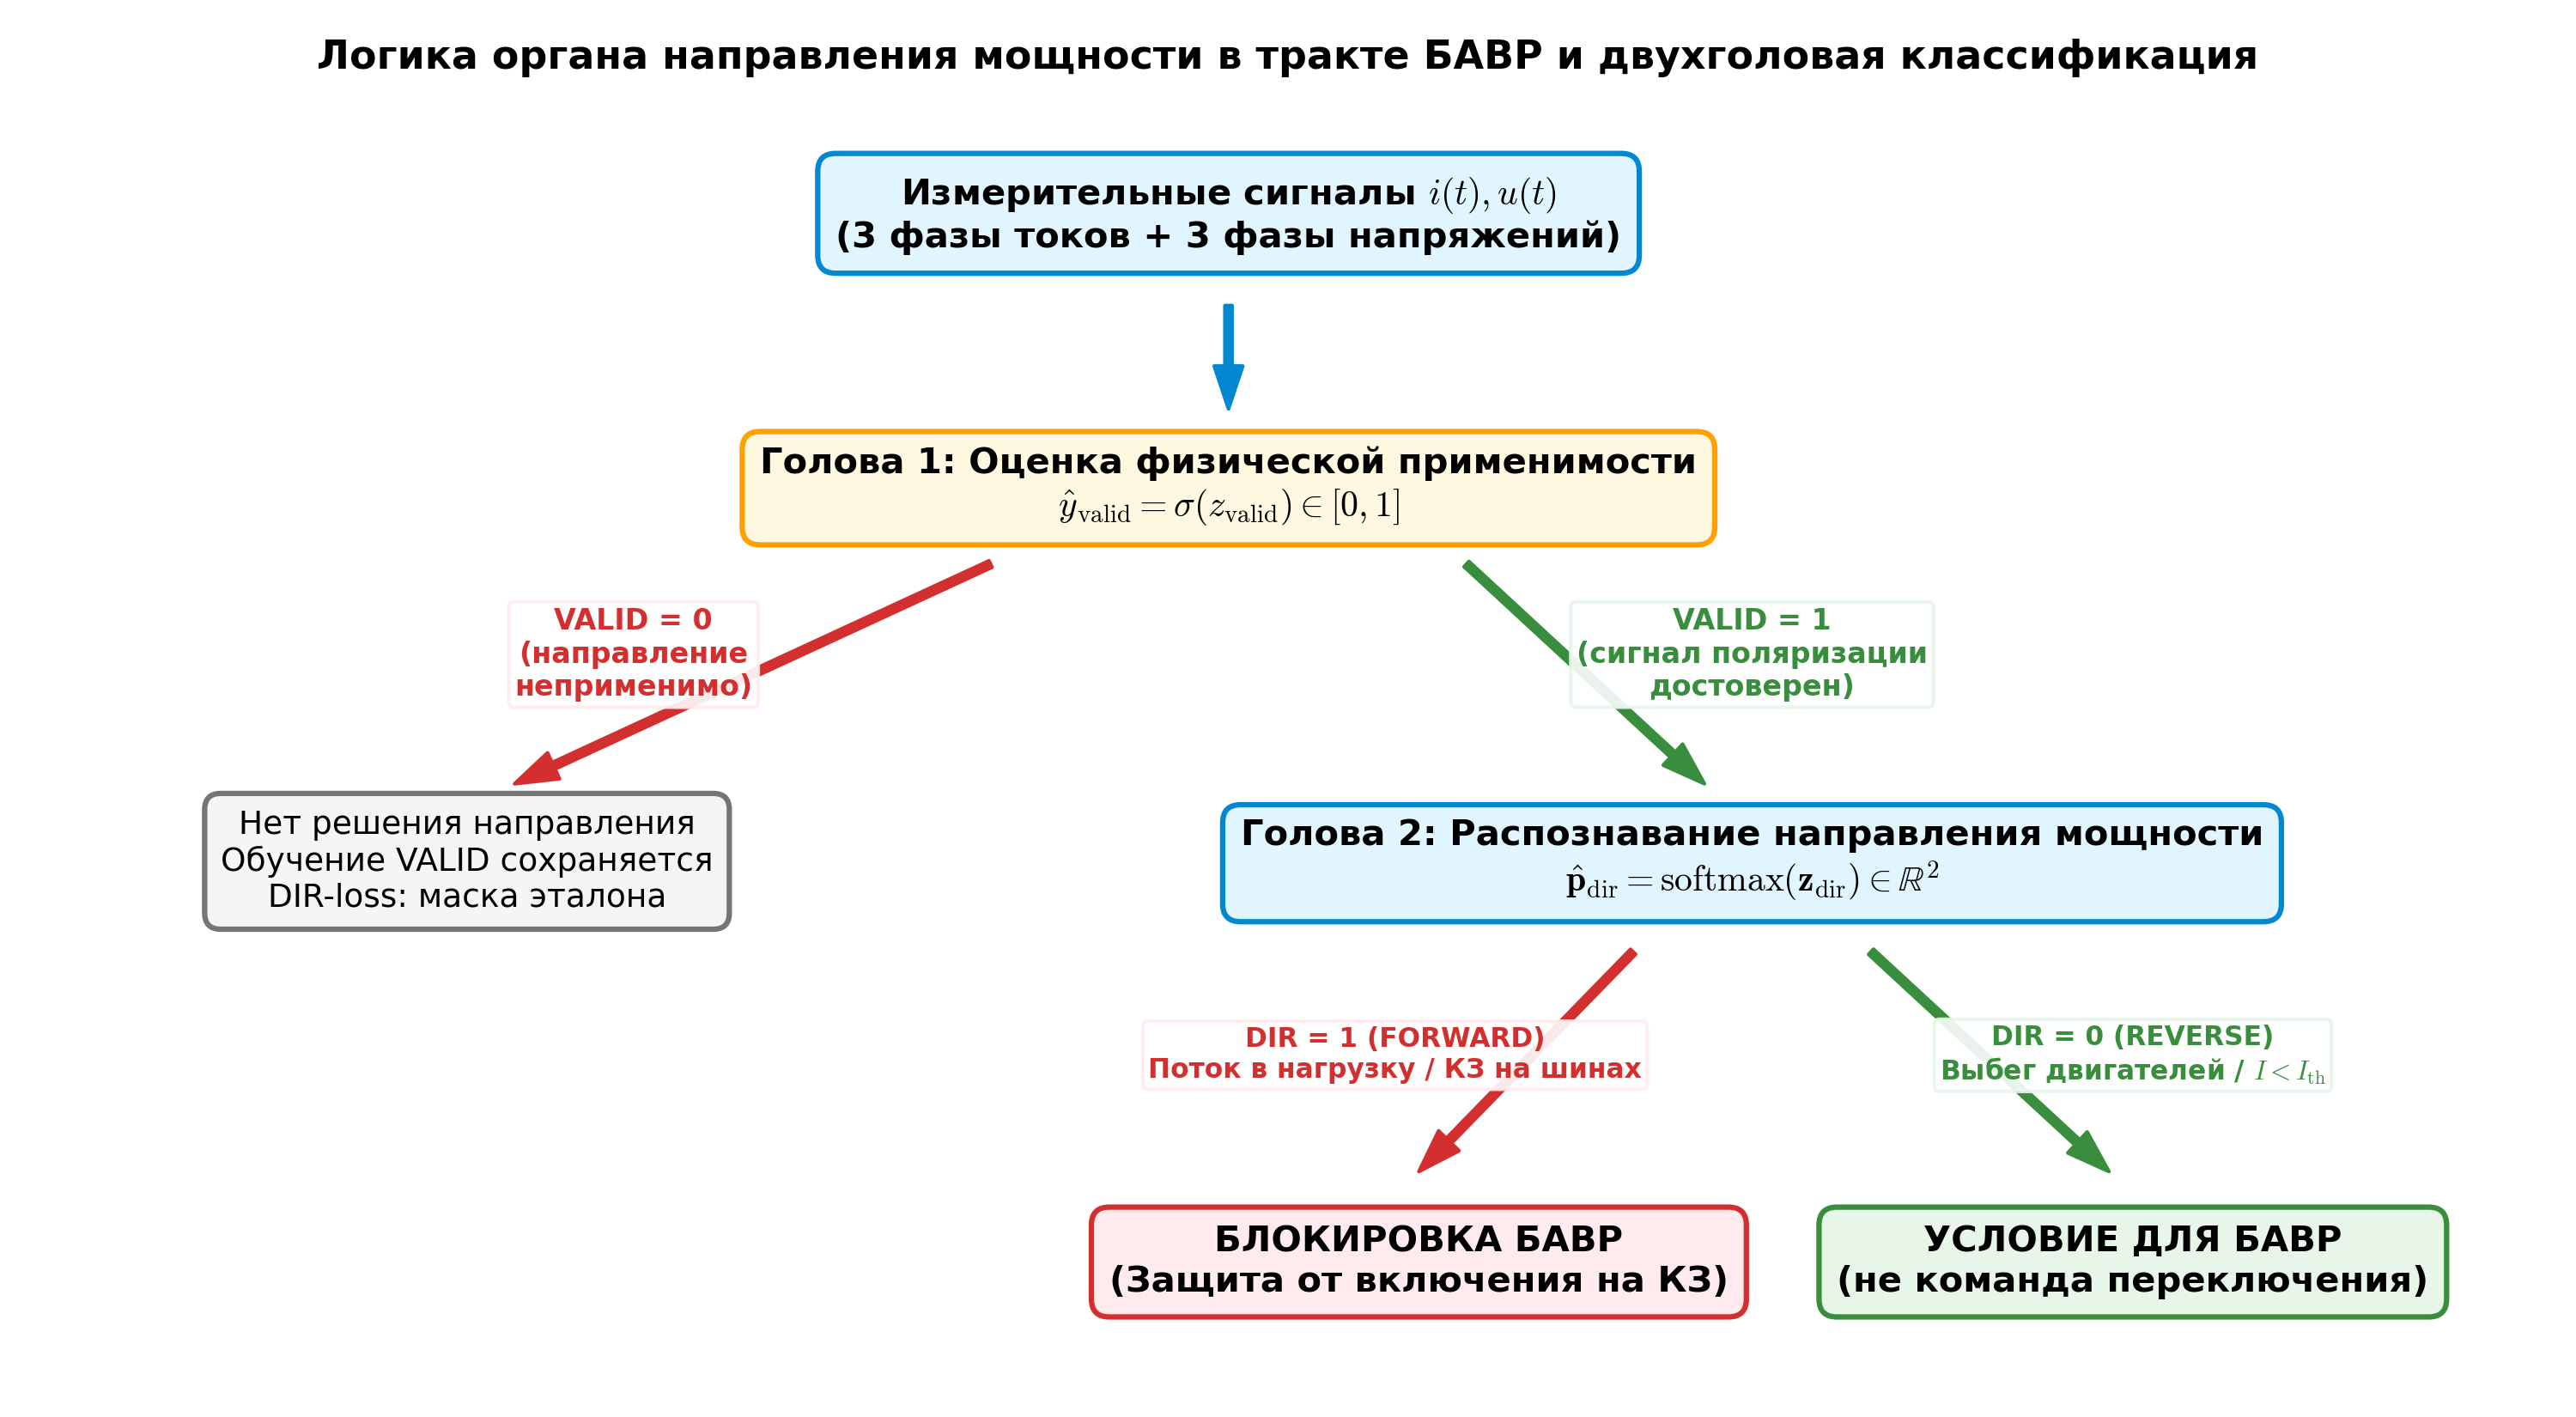
\includegraphics[width=\textwidth]{figures/ch05/ch05_bavr_twohead_article.png}
 \caption{Разделение оценки применимости
 и направления мощности в задаче БАВР}
 \label{fig:ch5_twohead_logic}
\end{figure}
\figurereview{Исходный рисунок 1 статьи 5. Схема показывает
логический порядок интерпретации, а не обязательное
последовательное вычисление двух голов. При следующей редакции
согласовать DIR=0 с текстом о подпороговом токе: это также
отсутствие блокировки, не только физически обратный поток.}

Обучение направления использует интервалы,
на которых оно определено в целевой разметке.
При неприменимом контексте сохраняется
задача оценки применимости,
а направление не используется
как достоверная обучающая цель.
В проверке эти два результата
также оцениваются отдельно.

Такое построение позволяет различать
ошибку направления и отказ от решения.
Оно не гарантирует автоматического
выявления всех неисправностей измерения.
Способность распознавать конкретные
неприменимые режимы определяется
их представленностью в данных
и отдельной предметной проверкой.

Полученный ответ РНМ относится
к состоянию измерительного органа.
Его использование для блокировки
или дальнейшей оценки условий БАВР
сохраняет принятую внешнюю логику
действия автоматики.
